%! Author = Main
%! Date = 05.02.2020

% Preamble
\documentclass{beamer}
\usetheme{Darmstadt}

% Packages
\usepackage{ngerman}
\usepackage{color} % Colored font
\usepackage{graphicx} % Images
\usepackage{titling} % Title formatting
\usepackage[utf8]{inputenc} % UTF-8
\usepackage {tikz}
\usepackage{amsmath} % Graphs
\usepackage{etoolbox} % Well formatted Links in bib
\apptocmd{\thebibliography}{\raggedright}{}{} % Well formatted Links in bib
\usepackage{hyperref} % Links

% Meta information
\title{\Huge{Intelligente Systeme}}
\subtitle{\Large - Referat -}
\author{Adrian Helberg}
\institute{HAW Hamburg}
\date{21.02.2020}
\titlegraphic{
\begin{picture}
    (0,0)
    % -56,20: Bottom left
    \put(-56,212){\makebox(0,0)[rt]{
\includegraphics[width=3.8cm]{../../resources/Haw_logo.png}}}
    \put(158,200){\makebox(0,0)[rt]{
\includegraphics[width=5cm]{../../resources/fakultaet.PNG}}}
\end{picture}
}

\newenvironment<>{definition}[1]{%
    \setbeamercolor{block title}{fg=white,bg=green!75!black}%
    \begin{block}#2{#1}}{\end{block}}

% Slides
\begin{document}
    \nocite{*} % List bibliography without even citing
    \frame{\titlepage}

    \frame{
    \frametitle{Inhalt}
    \tableofcontents
    }

    \AtBeginSection[]
    {
        \frame {
            \frametitle{Inhalt}
            \tableofcontents[currentsection]
        }
    }

    \section{Suchen}
    \frame{
    \frametitle{Problem des Handlungsreisenden}
        \begin{definition}{Definition}
            Die Aufgabe besteht darin, eine Reihenfolge für den Besuch mehrerer Orte so zu wählen,
            dass keine Station außer der ersten mehr als einmal besucht wird, die gesamte
            Reisestrecke des Handlungsreisenden möglichst kurz und die erste Station gleich der
            letzten Station ist \footnotemark
        \end{definition}
        \footnotetext[1]{\url{https://de.wikipedia.org/wiki/Problem_des_Handlungsreisenden}}

        \begin{itemize}
            \setlength\itemsep{0.6em}
            \item Kombinatorisches Optimierungsproblem
            \item $10!=3628800$ mögliche Lösungen
            \item Theoretische Informatik
            \item Festlegung der Reihenfolge der zu besuchenden Städte
            \item NP-vollständig
        \end{itemize}
    }

    \frame{
        \frametitle{Genetischer Algorithmus}
        \begin{definition}{Definition}
            Evolutionäre Algorithmen (EA) sind eine Klasse von stochastischen, metaheuristischen
            Optimierungsverfahren, deren Funktionsweise von der Evolution natürlicher Lebewesen
            inspiriert ist \footnotemark
        \end{definition}
        \footnotetext[2]{\url{https://de.wikipedia.org/wiki/Evolutionarer_Algorithmus}}

        \begin{itemize}
            \setlength\itemsep{1em}
            \item Optimierte, akzeptable Lösung
            \item Aufgabenstellung mit hoher kombinatorischen Komplexität
            \item Mengen an (immer besser werdenden) Lösungen
            \item Kein "`Hängenbleiben"' an einem lokalen Optimum
        \end{itemize}
    }

    \frame{
        \frametitle{Ablauf (1/2)}
        \begin{center}
            \begin{tikzpicture}[semithick , state/.style ={ rectangle ,top color =white , bottom color = processblue!20 ,
            draw,processblue , text=blue , minimum width =1 cm}]
                \node[state] (A) at (0,0) {Start};
                \node[state] (B) at (0,-1.2) {Erzeugung einer zufälliger Population};
                \node[state] (C) at (0,-2.4) {Wiederhole bis Abbruchbedungung erfüllt};
                \node[state] (D) at (0,-3.6) {Berechne Fitness};
                \node[state] (E) at (0,-4.8) {Selektion};

                \draw[->, very thick] (A) to (B);
                \draw[->, very thick] (B) to (C);
                \draw[->, very thick] (C) to (D);
                \draw[->, very thick] (D) to (E);
            \end{tikzpicture}
        \end{center}
    }

    \frame{
        \frametitle{Ablauf (2/2)}
        \begin{center}
            \begin{tikzpicture}[semithick , state/.style ={ rectangle ,top color =white , bottom color = processblue!20 ,
            draw,processblue , text=blue , minimum width =1 cm}]
                \node[state] (F) at (0,0) {Crossover};
                \node[state] (G) at (0,-1.2) {Mutation};
                \node[state] (H) at (0,-2.4) {Austausch};
                \node[state] (I) at (0,-3.6) {Teste Abbruchbedingung};
                \node[state] (J) at (0,-4.8) {Ende};

                \draw[->, very thick] (F) to (G);
                \draw[->, very thick] (G) to (H);
                \draw[->, very thick] (H) to (I);
                \draw[->, very thick] (I) to (J);
            \end{tikzpicture}
        \end{center}
    }

    \frame{
        \frametitle{Eigenschaften}
        \begin{itemize}
            \setlength\itemsep{1.6em}
            \item Chromosomen
            \item Fitness
            \item Selektion
            \item Kreuzung
            \item Mutation
            \item Austausch
        \end{itemize}
    }

    \frame{
        \frametitle{Realisierung mit Java}
        \begin{center}
            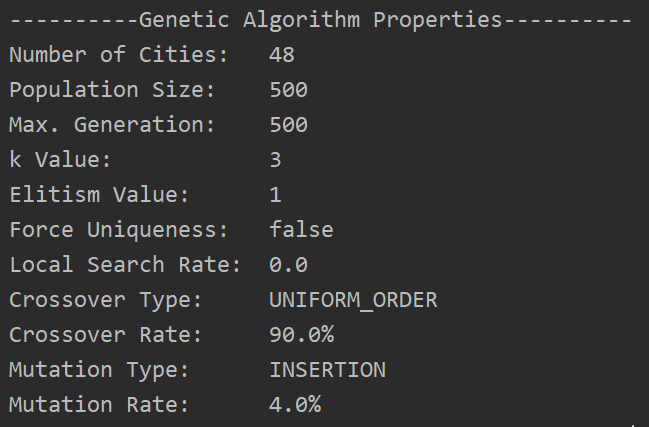
\includegraphics[width=10cm]{../../resources/properties_algorithm.png}
        \end{center}
    }

    \AtBeginSection[]
    {
        \frame {
            \frametitle{Inhalt}
            \tableofcontents[currentsection]
        }
    }

    \section{Lernen}
    \frame{
        \frametitle{Selbstorganierende Karte}
        \begin{definition}{Definition}
            Als Selbstorganisierende Karten $[...]$ bezeichnet man eine Art von künstlichen
            neuronalen Netzen. $[...]$ Ihr Funktionsprinzip beruht auf der biologischen Erkenntnis,
            dass viele Strukturen im Gehirn eine lineare oder planare Topologie aufweisen
            \footnotemark
        \end{definition}
        \footnotetext[3]{\url{https://de.wikipedia.org/wiki/Selbstorganisierende_Karte}}

        \begin{itemize}
            \setlength\itemsep{0.6em}
            \item Neuroinformatik
            \item \textit{Kohonen}-Karte, \textit{SOM}
            \item Unüberwachtes Lernen
        \end{itemize}
    }

    \frame{
        \frametitle{Prinzip}
        \begin{figure}
            \centering
            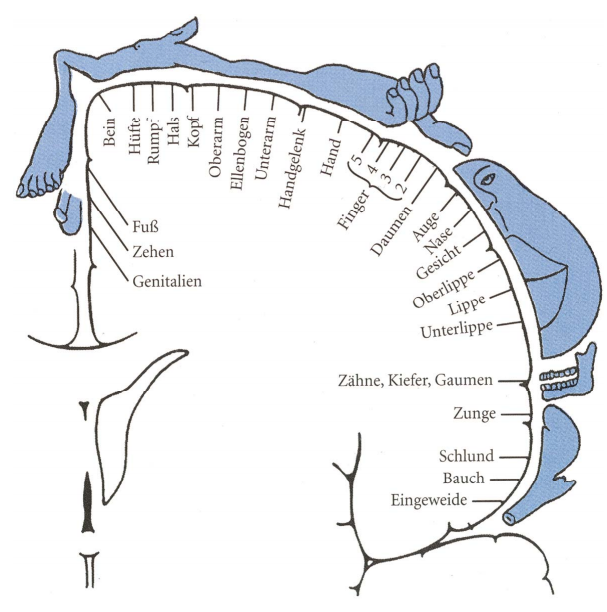
\includegraphics[width=6cm]{../../resources/gehirn.png}
            \caption{Topologische Abbildung des sensorischen Kortex}
        \end{figure}
    }

    \frame{
    \frametitle{Neuron}
        \begin{figure}
            \centering
            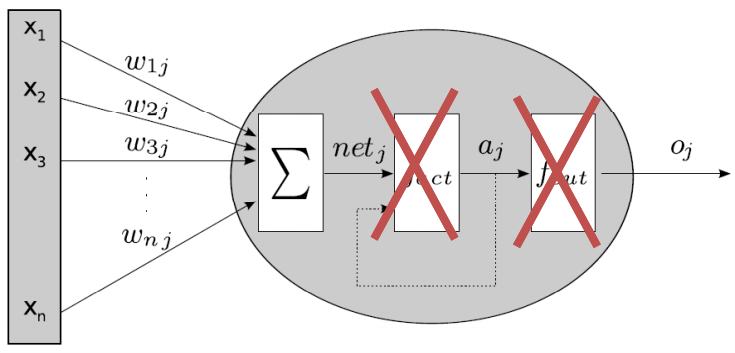
\includegraphics[width=8cm]{../../resources/neuron.png}
            \caption{Neuron einer \textit{SOM}}
        \end{figure}
        \begin{itemize}
            \setlength\itemsep{0.6em}
            \item Keine Aktivierungsfunktion
            \item Kein Mappingfunktion (Oputput)
        \end{itemize}
    }

    \frame{
        \frametitle{Neuron}
        \begin{figure}
            \centering
            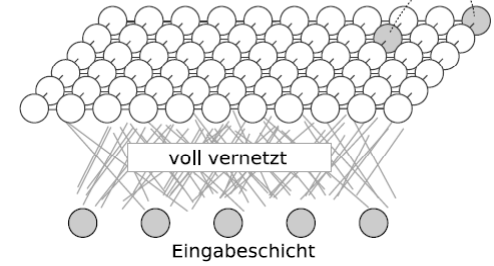
\includegraphics[width=8cm]{../../resources/netz.png}
            \caption{\textit{Kohonen}-Netz}
        \end{figure}
        \begin{itemize}
            \item Eingabeneuronen sind über die Gewichtsvektoren mit den Ausgabeneuronen
                  vollvermascht
        \end{itemize}
    }

    \frame{
        \frametitle{Lernen}
        \begin{itemize}
            \setlength\itemsep{1em}
            \item Auswahl von Neuronen über die "`Eignung"' (euklidische Norm)
            \item Abstand zwischen Eingabevektoren und Gewichtvektoren wird bestimmt
            \item Zufällige Auswahl bei gleicher Distanz
            \item \textit{Besonderes}: "`Sigerneuron"' \textbf{und} dessen Nachbarneuronen werden
                angepasst
        \end{itemize}
    }

    \frame{
        \frametitle{Distanzfunktionen}
        \begin{figure}
            \centering
            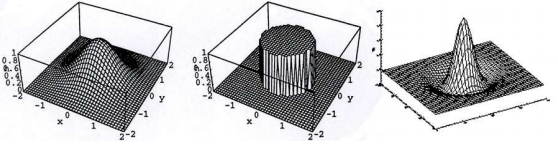
\includegraphics[width=10cm]{../../resources/distanzfunktionen.png}
            \caption{Gaussche Glockenfunktion, Zylinderfunktion und "`Mexican-Hat"'}
        \end{figure}
    }

    \frame{
        \frametitle{Anpassen}
        \begin{block}{Siegerneuron anpassen}
            $W_c = W_c + \Delta W_c$ und $\Delta W_c = \eta * (x-W_c)$, mit
            \begin{itemize}
                \item $c$ als Siegerneuron
                \item $W_c$ als Gewichtungsvektor
                \item Eingabevektor $x$
            \end{itemize}
            Es gilt $0 < \eta < 1$.
        \end{block}
    }

    \frame{
        \frametitle{Anpassen}
        \begin{block}{Nachbarneuronen anpassen}
            $\Delta W_j = \eta * h_c_j * (x - W_j)$, mit
            \begin{itemize}
                \item $h_c_j$ als Nachbarschaftsfunktion (Wie stark lernt das Neuron $j$ mit bei Siegerneuron $c$)
            \end{itemize}
        \end{block}\\~\\
        Als Funktion des Abstandes $z$ der Neuronen wird in der Praxis oft eine Zylinderfunktion
        gewählt:\\~\\
        $Zylinder: h_c_j(z) =
        \begin{cases}
            1 & falls \; z < d\\
            0 & sonst.
        \end{cases}$
    }

    \frame{
        \frametitle{Lernmetapher}
        \begin{definition}{"`Kupferschmiede"'}
            Ein Kupferschmied hämmert auf einer Kupferplatte. Hierbei bestimmt
            \begin{itemize}
                \item der Vektor $x$, wohin
                \item die Lernrate $\eta$, wie stark
                \item der Lernradius $d$, mit welcher Hammergröße und
                \item die Nachbarschaftsfunktion $h_c_j$, mit welcher Hammerform geschlagen wird
            \end{itemize}
        \end{definition}
    }

    \frame{
        \frametitle{Anwendung - Fragestellung}
        \begin{figure}
            \centering
            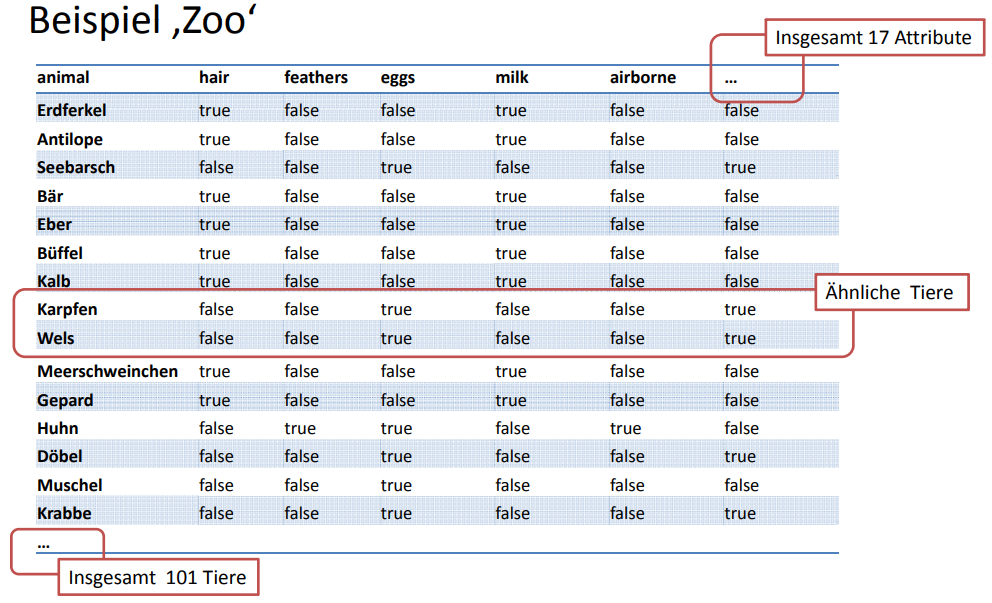
\includegraphics[width=10cm]{../../resources/zoo_table.png}
            \caption{Sind ähnliche Tiere eines Zoos benachbart?}
        \end{figure}
    }

    \frame{
    \frametitle{Anwendung - Resultierende Map}
    \begin{figure}
        \centering
        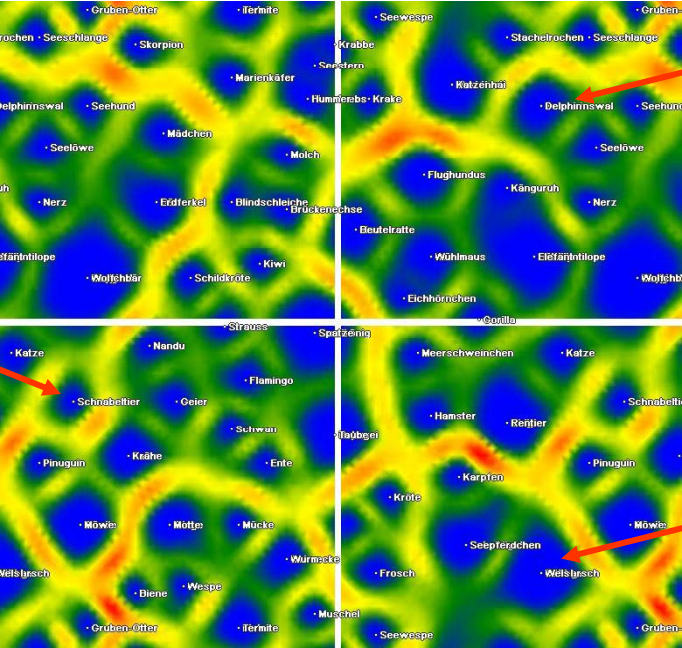
\includegraphics[width=6.8cm]{../../resources/zoo.png}
        \caption{Reduktion mehrerer Dimensionen auf 2 (Karte)}
    \end{figure}
    }

    \frame{
    \frametitle{Anwendung - Anwendungsgebiete}
    \begin{itemize}
        \setlength\itemsep{1em}
        \item Dimensionsreduktion
        \item Optimierung
        \item Data Mining - Cluster
        \item Data Mining - Regeln
        \item Überwachung und Anomaliedetektion
        \item Kontextkarten
    \end{itemize}
    }

    \AtBeginSection[]
    {
        \frame {
            \frametitle{Inhalt}
            \tableofcontents[currentsection]
        }
    }

    \section{Sequenzen}
    \frame{
    \frametitle{Thema}
        \begin{definition}{Verarbeitung mobiler Sensordaten}
            \begin{itemize}
                \setlength\itemsep{1em}
                \item Steigende Beliebtheit tragbarer Endgeräte
                \item Kontinuierliche Erfassung physiologischer und funktioneller Daten
                \item Anwendungen bei Apps für Sport, Gesundheit und Wohlbefinden
                \item Verarbeitung und Analyse von \textbf{Big Data}
                \item \textit{Deep Learning}- Ansatz
            \end{itemize}
        \end{definition}
    }

    \frame{
    \frametitle{Thema}
    \begin{definition}{\textit{Human Activity Recognition} (HAR)}
        \begin{itemize}
        \setlength\itemsep{1em}
            \item Auswertung zeitlicher Reihendaten von Trägheitssensoren
            \item Identifikation ausgeführter Aktionen: Klassifizierung von Bewegungsabläufen
            \item Erkennung von Krankheitsausbrüchen (z.B. Parkinson) oder Wirksamkeit einer
                Behandlung
        \end{itemize}
    \end{definition}
    }

    \frame{
        \frametitle{Problem}
        \begin{itemize}
            \setlength\itemsep{1em}
            \item \textit{Deep Learning} ist zur Zeit sehr erfolgreich bei Implementationen, die
                Hochleistungs-Rechencluster nutzen.
            \item Einsatz auf mobilen Endgeräten stellt sich als schwierig heraus, da nur geringe
                Ressourcen zur Verfügung stehen
            \item Gesucht ist ein optimiertes Verfahren: Bestes Ergebnis bei geringsten Ressourcen
        \end{itemize}
    }

    \frame{
        \frametitle{Technik}
        \begin{itemize}
            \setlength\itemsep{1em}
            \item Entwerfen der Klassifizierungsmethode für eine Zeitreihenanalyse
            \item Auswahl von Merkmalen der Klassen
            \item Oft durch den Einsatz von \textit{Deep Believe Networks} (DBN),
                \textit{Restricted Boltzman Machines} (RBM) oder
                \textit{Convolutional Neural Networks} (CNN) umgesetzt
            \item Herausarbeiten von \textit{Features} aus Rohdaten
        \end{itemize}
    }

    \frame{
        \frametitle{"`Shallow Deep Learning"'- Methode}
        \begin{definition}{Prinzip}
            \textit{Shallow Deep Learning} setzt sich aus \textit{Deep Learning} und
            \textit{Shallow Learning} zusammen und ist für \textit{HAR} unterteilt in:
            \begin{itemize}
                \setlength\itemsep{0.8em}
                \item Input
                \item Segmentextraktion
                \item Spektorgramm
                \item \textit{Deep Learning} Modul
                \item \textit{Shallow Features}
                \item Training
                \item Evaluation
            \end{itemize}
        \end{definition}
    }

    \frame{
        \frametitle{Ablauf}
        \begin{figure}
            \centering
            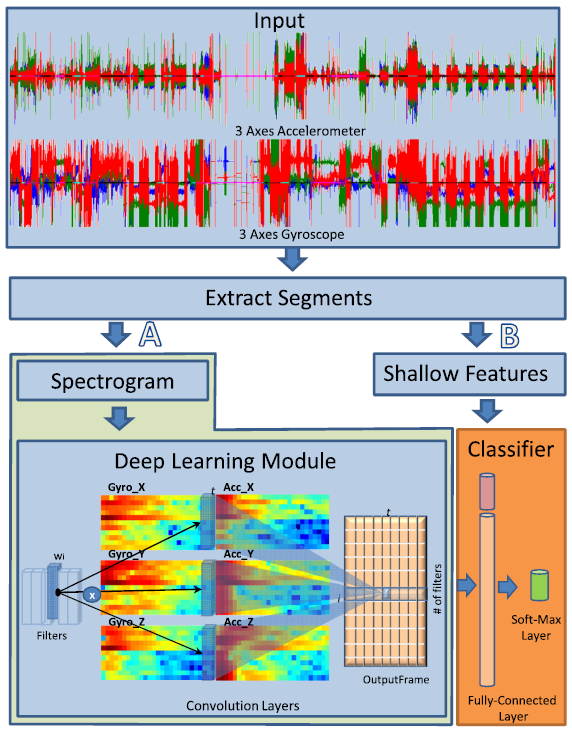
\includegraphics[width=5cm]{../../resources/prozess.png}
            \caption{Schamatischer Ablauf}
        \end{figure}
    }

    \frame{
        \frametitle{Prozess}
        \begin{block}{Input}
            Um eingehende Daten (Input) zu generieren wird auf verbaute Trägheitssensoren wie
            \begin{itemize}
                \item Beschleunigungsmesser und
                \item Gyroskope
            \end{itemize}
            zugegriffen. Zugriffe auf anderen Sensoren, wie Elektrokardiographie (EKG)
            oder Elektromyographie (EMG), sind ebenfalls möglich (Smartwatch)
        \end{block}
    }

    \frame{
        \frametitle{Prozess}
        \begin{block}{Segmente extrahieren}
            \begin{itemize}
                \item Extraktion von $n$ Segmenten aus den Rohdaten ($n$ hängt von der Art der Anwendung ab)
                \item Segmente bei \textit{HAR} werden auf 4 bis 10 Sekunden (\textit{sliding window}) gesetzt
                \begin{itemize}
                    \item Genauigkeit der Erkennung der ausgeführten Aktivität soll maximal sein
                    \item Verschleierung der Grenzen zwischen verschiedenen Aktivitäten soll
                        minimal sein
                \end{itemize}
            \end{itemize}
        \end{block}
    }

    \frame{
    \frametitle{Prozess}
        \begin{block}{Spektogramm}
            \begin{itemize}
                \item Segmente werden als Spektogramm-Repräsentation an das \textit{Deep Learning} Modul weitergereich
                \item Herausarbeiten von Intensitätsunterschieden in den Trägheitspunkten des Spektogramms, wie
                \begin{itemize}
                    \item Zeit- und Abtastrateninvarianz
                    \item Amplituden
                    \item Frequenz
                \end{itemize}
            \end{itemize}
        \end{block}
    }

    \frame{
        \frametitle{Prozess}
        \begin{figure}
            \centering
            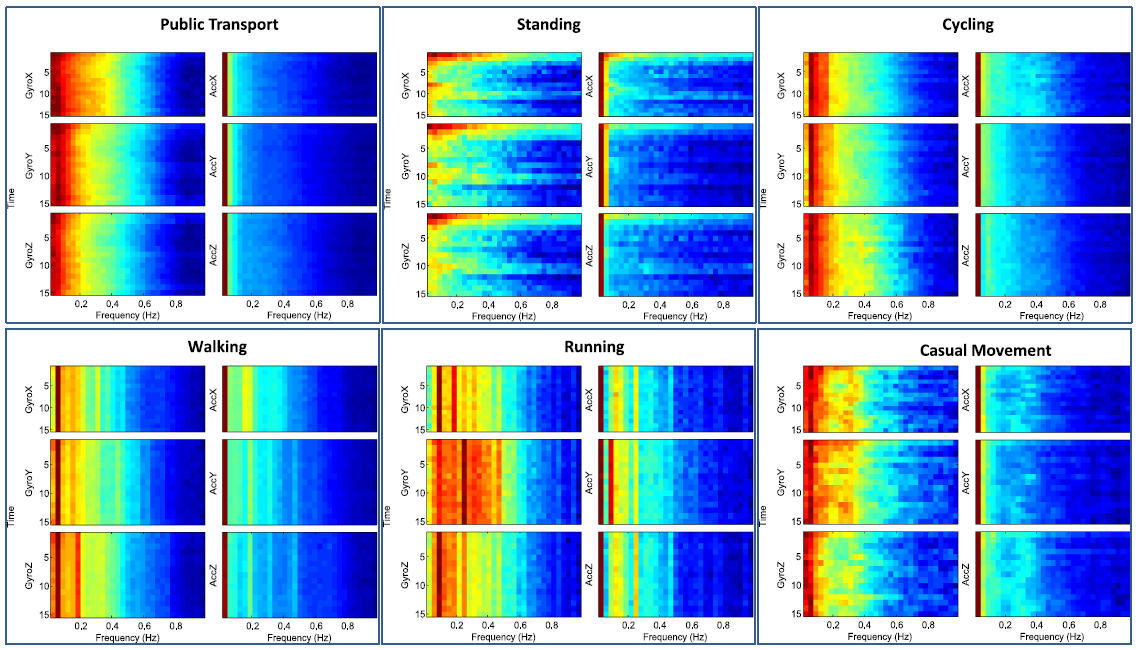
\includegraphics[width=10.8cm]{../../resources/features.png}
            \caption{Spektorgramme aus verschiedenen Aktivitäten}
        \end{figure}
    }

    \frame{
        \frametitle{Prozess}
        \begin{block}{Shallow Features}
            Intensitätsunterschiede in den Spektogrammen ergeben "`flache"' Merkmale, die auf die Spektogramme
            angewendet werden. Beispiele sind
            \begin{itemize}
                \item Quadratischer Mittelwert
                \item Standartabweichung
            \end{itemize}
        \end{block}
        \begin{block}{Klassifizierung}
            Sobald sowohl flache ("`shallow learned"'), als auch tiefe ("`deep learned"') Eigenschaften berechnet wurden, können diese zu einem eindeutigen Vektor
            zusammengeführt und klassifiziert werden
        \end{block}
    }

    \frame{
        \frametitle{Prozess}
        \begin{block}{Training}
            Flache und tiefe Features werden zusammen in einem einheitlichen, neuronalem Netz trainiert.
            In jeder Schicht des neuronalen Netzes werden Fehler
            (Errors) zwischen den Soll- und Istwerten in einer \textit{Backwards Propagation}-
            Routine genutzt, um die Gewichtungen in den \textit{Hidden-Layers} anzupassen.
        \end{block}
        \begin{block}{Evaluation}
            Das vorgeschlagene \textit{Shallow Deep Learning}-Verfahren könnte nun mit verschiedenen
            Datensätzen analysiert und evaluiert werden
        \end{block}
    }

    \frame{
        \frametitle{Prozess}
        \begin{figure}
            \centering
            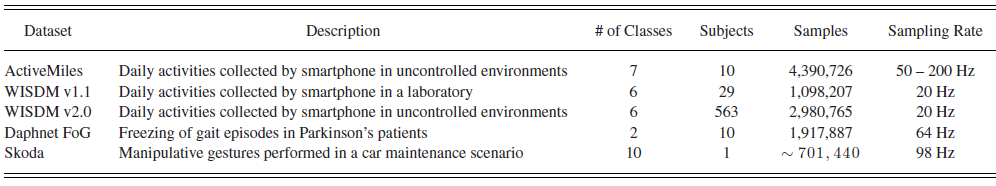
\includegraphics[width=11cm]{../../resources/datasets.png}
            \caption{Datensätze für eine Evaluierung}
        \end{figure}
    }

    \AtBeginSection[]
    {
        \frame {
            \frametitle{Inhalt}
            \tableofcontents[currentsection]
        }
    }

    \section{Quellen}
    \frame[allowframebreaks]{
    \frametitle{Quellen}
        \bibliographystyle{plain}
        \bibliography{script}
    }

    \frame{
    \frametitle{Danksagung}
    \begin{center}
        Danke für die Aufmerksamkeit!
    \end{center}
    }

\end{document}